%	Preamble. Put stuff here to define global settings.
% SJK: Document template originally from Andy Maloney "untitled.tex"
\documentclass{article}

%	Packages used.
\usepackage{amsmath}
\usepackage{fullpage}
\usepackage{graphicx}
\usepackage{caption}
\usepackage{subcaption}
%% see: http://en.wikibooks.org/wiki/LaTeX/Floats,_Figures_and_Captions#Subfloats
%	Define new commands for fun and expediated typing.
\newcommand{\bdm}{\begin{displaymath}}
\newcommand{\edm}{\end{displaymath}}

\begin{document}
	Quick summary of ridge regression (3.1.2 Ridge Regression).

	\begin{itemize}
		\item Following the beginning of supervised learning, simple least-squares is easy (and probably usually wrong).  The next example is plot\_ridge\_path.html I replicated the code, learned a bit, but am still not clear on how ridge regression works, but I'm going to move on.
	\end{itemize}

    \begin{figure}
            \centering
            \begin{subfigure}[b]{0.3\textwidth}
                    \centering
                    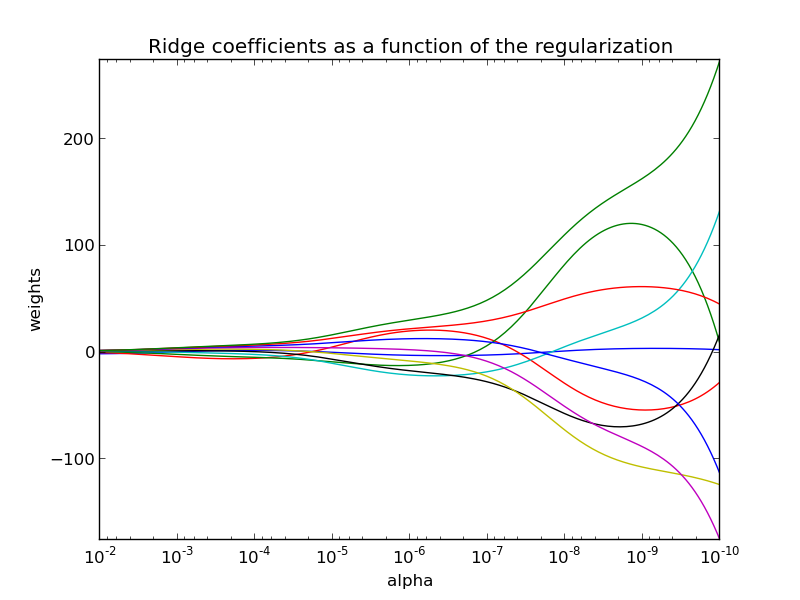
\includegraphics[width=\textwidth]{fig_original.png}
                    \caption{Original figure, 10x10 Hilbert, y=ones(10)}
                    \label{fig:orig}
            \end{subfigure}%
            ~ %add desired spacing between images, e. g. ~, \quad, \qquad etc.
              %(or a blank line to force the subfigure onto a new line)
            \begin{subfigure}[b]{0.3\textwidth}
                    \centering
                    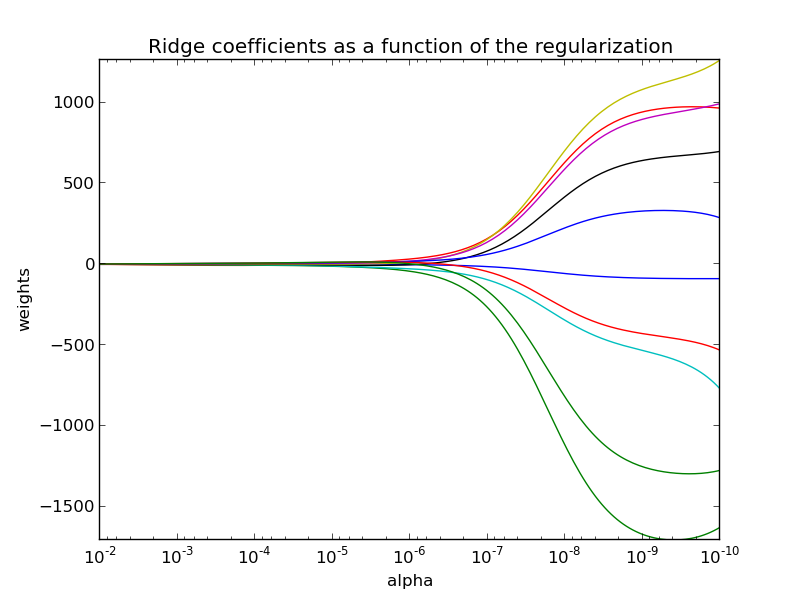
\includegraphics[width=\textwidth]{fig_yrand.png}
                    \caption{10x10 Hilbert, y = rand(10)}
                    \label{fig:yrand}
            \end{subfigure}
            ~ %add desired spacing between images, e. g. ~, \quad, \qquad etc.
              %(or a blank line to force the subfigure onto a new line)
            \begin{subfigure}[b]{0.3\textwidth}
                    \centering
                    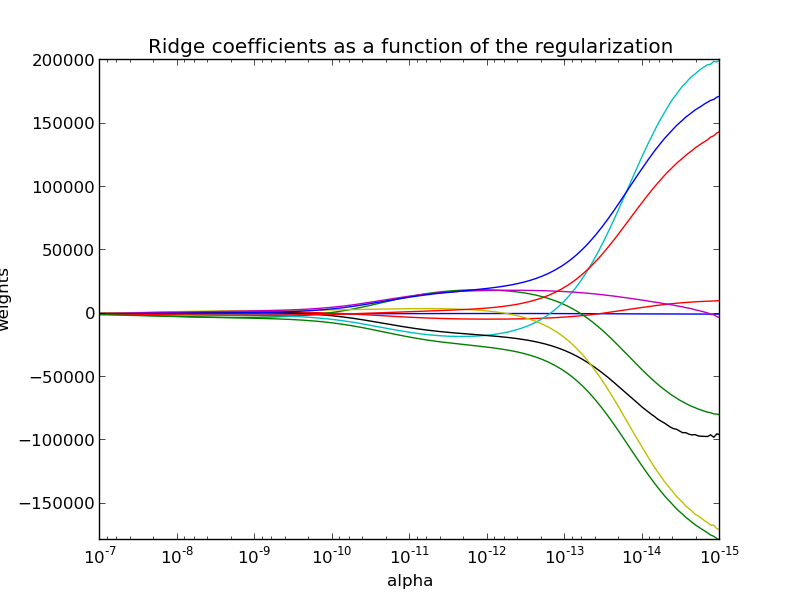
\includegraphics[width=\textwidth]{fig_y10to1.png}
                    \caption{10x10 Hilber, y = 10, 9, 8, ..., 1}
                    \label{fig:y10to1}
            \end{subfigure}
            \caption{Ridge regression with three different y arrays}\label{fig:images3}
    \end{figure}


\end{document}
